\documentclass{standalone}
\usepackage{tikz}
\usetikzlibrary{patterns, positioning}


\begin{document}
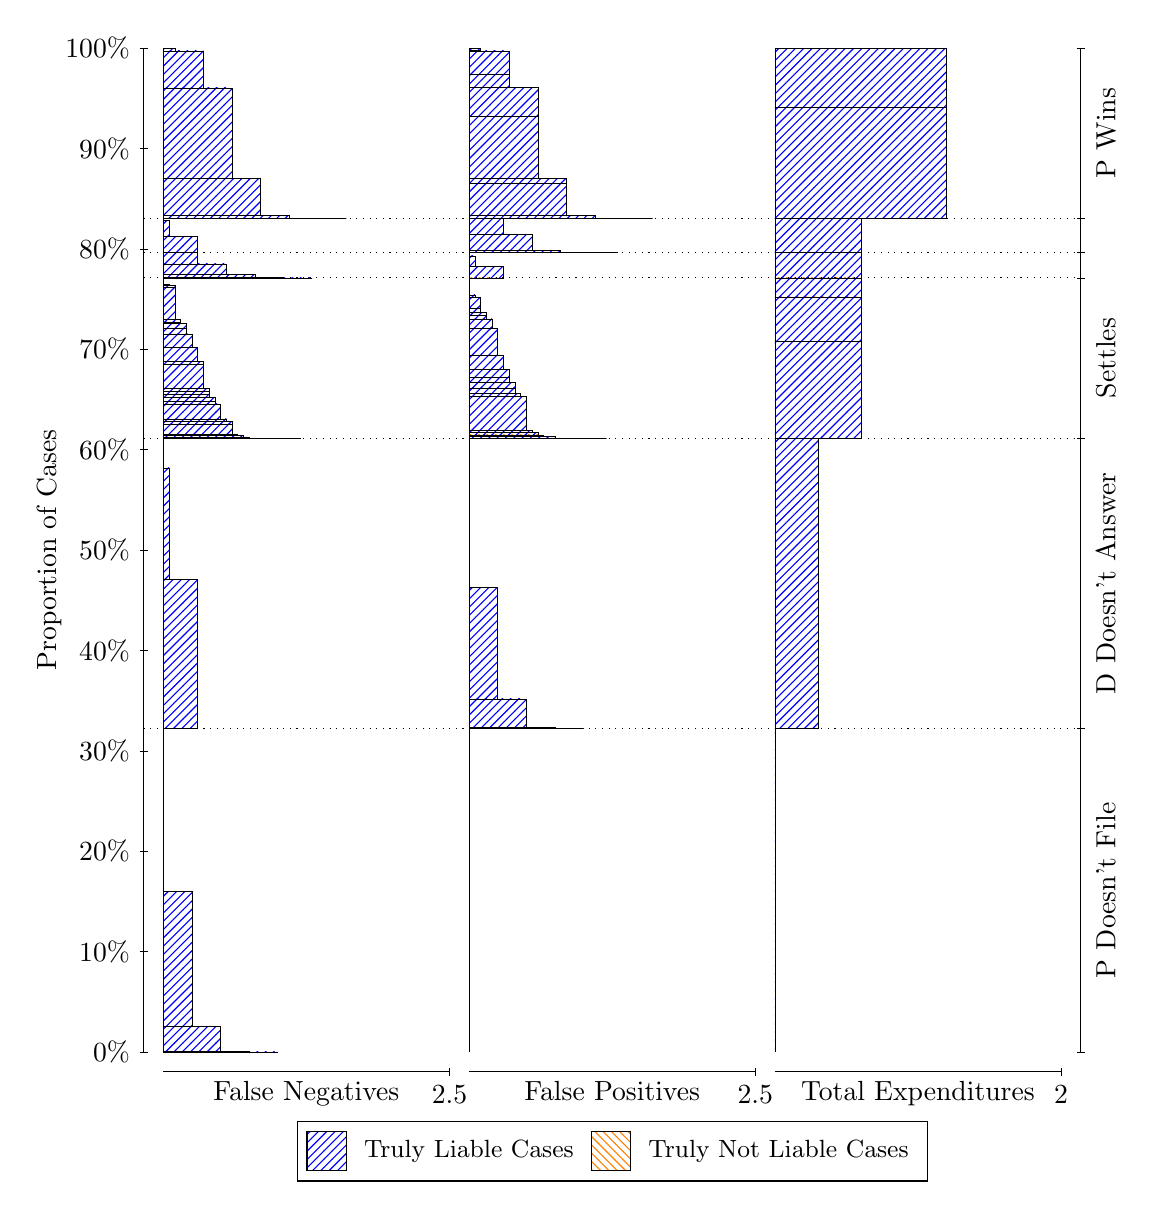
\begin{tikzpicture}
\draw[black, very thin] (1.5,1.75) -- (1.5,14.5);
\node[rotate=90, text=black, anchor=center] at (0.3, 8.125) {Proportion of Cases};
\draw[black, very thin] (1.45,1.75) -- (1.55,1.75);
\node[text=black, anchor=east] at (1.45, 1.75) {0\%};
\draw[black, very thin] (1.45,3.025) -- (1.55,3.025);
\node[text=black, anchor=east] at (1.45, 3.025) {10\%};
\draw[black, very thin] (1.45,4.3) -- (1.55,4.3);
\node[text=black, anchor=east] at (1.45, 4.3) {20\%};
\draw[black, very thin] (1.45,5.575) -- (1.55,5.575);
\node[text=black, anchor=east] at (1.45, 5.575) {30\%};
\draw[black, very thin] (1.45,6.85) -- (1.55,6.85);
\node[text=black, anchor=east] at (1.45, 6.85) {40\%};
\draw[black, very thin] (1.45,8.125) -- (1.55,8.125);
\node[text=black, anchor=east] at (1.45, 8.125) {50\%};
\draw[black, very thin] (1.45,9.4) -- (1.55,9.4);
\node[text=black, anchor=east] at (1.45, 9.4) {60\%};
\draw[black, very thin] (1.45,10.675) -- (1.55,10.675);
\node[text=black, anchor=east] at (1.45, 10.675) {70\%};
\draw[black, very thin] (1.45,11.95) -- (1.55,11.95);
\node[text=black, anchor=east] at (1.45, 11.95) {80\%};
\draw[black, very thin] (1.45,13.225) -- (1.55,13.225);
\node[text=black, anchor=east] at (1.45, 13.225) {90\%};
\draw[black, very thin] (1.45,14.5) -- (1.55,14.5);
\node[text=black, anchor=east] at (1.45, 14.5) {100\%};

\draw[black, very thin] (13.4,1.75) -- (13.4,14.5);
\draw[black, very thin] (13.35,1.75) -- (13.45,1.75);
\node[anchor=west] at (13.35, 1.75) {};
\draw[black, very thin] (13.35,5.858) -- (13.45,5.858);
\node[anchor=west] at (13.35, 5.858) {};
\draw[black, very thin] (13.35,9.5429) -- (13.45,9.5429);
\node[anchor=west] at (13.35, 9.5429) {};
\draw[black, very thin] (13.35,11.581) -- (13.45,11.581);
\node[anchor=west] at (13.35, 11.581) {};
\draw[black, very thin] (13.35,11.907) -- (13.45,11.907);
\node[anchor=west] at (13.35, 11.907) {};
\draw[black, very thin] (13.35,12.34) -- (13.45,12.34);
\node[anchor=west] at (13.35, 12.34) {};
\draw[black, very thin] (13.35,14.5) -- (13.45,14.5);
\node[anchor=west] at (13.35, 14.5) {};

\draw[black, very thin, pattern color=blue, pattern=north east lines] (1.75,1.75) rectangle (3.2033,1.75);
\draw[black, very thin, pattern color=blue, pattern=north east lines] (1.75,1.75) rectangle (2.84,1.7527);
\draw[black, very thin, pattern color=blue, pattern=north east lines] (1.75,1.7527) rectangle (2.4767,2.0758);
\draw[black, very thin, pattern color=blue, pattern=north east lines] (1.75,2.0758) rectangle (2.1133,3.7942);
\draw[black, very thin, pattern color=orange, pattern=north west lines] (1.75,3.7942) rectangle (1.75,3.7942);
\draw[black, very thin, pattern color=blue, pattern=north east lines] (1.75,3.7942) rectangle (1.75,5.858);
\draw[black, very thin, pattern color=blue, pattern=north east lines] (1.75,5.858) rectangle (2.186,7.7542);
\draw[black, very thin, pattern color=blue, pattern=north east lines] (1.75,7.7542) rectangle (1.8227,9.1666);
\draw[black, very thin, pattern color=orange, pattern=north west lines] (1.75,9.1666) rectangle (1.75,9.1666);
\draw[black, very thin, pattern color=blue, pattern=north east lines] (1.75,9.1666) rectangle (1.75,9.5429);
\draw[black, very thin, pattern color=blue, pattern=north east lines] (1.75,9.5429) rectangle (3.494,9.543);
\draw[black, very thin, pattern color=blue, pattern=north east lines] (1.75,9.543) rectangle (3.3487,9.543);
\draw[black, very thin, pattern color=blue, pattern=north east lines] (1.75,9.543) rectangle (3.2033,9.543);
\draw[black, very thin, pattern color=blue, pattern=north east lines] (1.75,9.543) rectangle (3.1307,9.5446);
\draw[black, very thin, pattern color=blue, pattern=north east lines] (1.75,9.5446) rectangle (3.058,9.5446);
\draw[black, very thin, pattern color=blue, pattern=north east lines] (1.75,9.5446) rectangle (3.058,9.5447);
\draw[black, very thin, pattern color=blue, pattern=north east lines] (1.75,9.5447) rectangle (2.9853,9.5467);
\draw[black, very thin, pattern color=blue, pattern=north east lines] (1.75,9.5467) rectangle (2.9127,9.5484);
\draw[black, very thin, pattern color=blue, pattern=north east lines] (1.75,9.5484) rectangle (2.84,9.5588);
\draw[black, very thin, pattern color=blue, pattern=north east lines] (1.75,9.5588) rectangle (2.7673,9.5822);
\draw[black, very thin, pattern color=blue, pattern=north east lines] (1.75,9.5822) rectangle (2.6947,9.5869);
\draw[black, very thin, pattern color=blue, pattern=north east lines] (1.75,9.5869) rectangle (2.6947,9.5939);
\draw[black, very thin, pattern color=blue, pattern=north east lines] (1.75,9.5939) rectangle (2.622,9.7279);
\draw[black, very thin, pattern color=blue, pattern=north east lines] (1.75,9.7279) rectangle (2.622,9.7587);
\draw[black, very thin, pattern color=blue, pattern=north east lines] (1.75,9.7587) rectangle (2.5493,9.7913);
\draw[black, very thin, pattern color=blue, pattern=north east lines] (1.75,9.7913) rectangle (2.4767,9.982);
\draw[black, very thin, pattern color=blue, pattern=north east lines] (1.75,9.982) rectangle (2.404,10.018);
\draw[black, very thin, pattern color=blue, pattern=north east lines] (1.75,10.018) rectangle (2.404,10.062);
\draw[black, very thin, pattern color=blue, pattern=north east lines] (1.75,10.062) rectangle (2.3313,10.102);
\draw[black, very thin, pattern color=blue, pattern=north east lines] (1.75,10.102) rectangle (2.3313,10.136);
\draw[black, very thin, pattern color=blue, pattern=north east lines] (1.75,10.136) rectangle (2.3313,10.178);
\draw[black, very thin, pattern color=blue, pattern=north east lines] (1.75,10.178) rectangle (2.2587,10.482);
\draw[black, very thin, pattern color=blue, pattern=north east lines] (1.75,10.482) rectangle (2.2587,10.525);
\draw[black, very thin, pattern color=blue, pattern=north east lines] (1.75,10.525) rectangle (2.186,10.703);
\draw[black, very thin, pattern color=blue, pattern=north east lines] (1.75,10.703) rectangle (2.1133,10.87);
\draw[black, very thin, pattern color=blue, pattern=north east lines] (1.75,10.87) rectangle (2.0407,10.94);
\draw[black, very thin, pattern color=blue, pattern=north east lines] (1.75,10.94) rectangle (2.0407,11.006);
\draw[black, very thin, pattern color=blue, pattern=north east lines] (1.75,11.006) rectangle (1.968,11.013);
\draw[black, very thin, pattern color=blue, pattern=north east lines] (1.75,11.013) rectangle (1.968,11.022);
\draw[black, very thin, pattern color=blue, pattern=north east lines] (1.75,11.022) rectangle (1.968,11.051);
\draw[black, very thin, pattern color=blue, pattern=north east lines] (1.75,11.051) rectangle (1.8953,11.462);
\draw[black, very thin, pattern color=blue, pattern=north east lines] (1.75,11.462) rectangle (1.8953,11.483);
\draw[black, very thin, pattern color=blue, pattern=north east lines] (1.75,11.483) rectangle (1.8227,11.503);
\draw[black, very thin, pattern color=orange, pattern=north west lines] (1.75,11.503) rectangle (1.75,11.503);
\draw[black, very thin, pattern color=blue, pattern=north east lines] (1.75,11.503) rectangle (1.75,11.581);
\draw[black, very thin, pattern color=blue, pattern=north east lines] (1.75,11.581) rectangle (3.6393,11.581);
\draw[black, very thin, pattern color=blue, pattern=north east lines] (1.75,11.581) rectangle (3.276,11.583);
\draw[black, very thin, pattern color=blue, pattern=north east lines] (1.75,11.583) rectangle (2.9127,11.627);
\draw[black, very thin, pattern color=blue, pattern=north east lines] (1.75,11.627) rectangle (2.5493,11.759);
\draw[black, very thin, pattern color=blue, pattern=north east lines] (1.75,11.759) rectangle (2.186,11.907);
\draw[black, very thin, pattern color=orange, pattern=north west lines] (1.75,11.907) rectangle (1.75,11.907);
\draw[black, very thin, pattern color=blue, pattern=north east lines] (1.75,11.907) rectangle (2.186,12.11);
\draw[black, very thin, pattern color=blue, pattern=north east lines] (1.75,12.11) rectangle (1.8227,12.314);
\draw[black, very thin, pattern color=orange, pattern=north west lines] (1.75,12.314) rectangle (1.75,12.314);
\draw[black, very thin, pattern color=blue, pattern=north east lines] (1.75,12.314) rectangle (1.75,12.34);
\draw[black, very thin, pattern color=blue, pattern=north east lines] (1.75,12.34) rectangle (4.0753,12.34);
\draw[black, very thin, pattern color=blue, pattern=north east lines] (1.75,12.34) rectangle (3.712,12.341);
\draw[black, very thin, pattern color=blue, pattern=north east lines] (1.75,12.341) rectangle (3.3487,12.376);
\draw[black, very thin, pattern color=blue, pattern=north east lines] (1.75,12.376) rectangle (2.9853,12.844);
\draw[black, very thin, pattern color=blue, pattern=north east lines] (1.75,12.844) rectangle (2.622,13.995);
\draw[black, very thin, pattern color=blue, pattern=north east lines] (1.75,13.995) rectangle (2.2587,14.464);
\draw[black, very thin, pattern color=blue, pattern=north east lines] (1.75,14.464) rectangle (1.8953,14.5);
\draw[black, very thin, pattern color=orange, pattern=north west lines] (1.75,14.5) rectangle (1.75,14.5);
\draw[black, very thin, pattern color=blue, pattern=north east lines] (1.75,14.5) rectangle (1.75,14.5);
\draw[black, very thin, pattern color=orange, pattern=north west lines] (5.6333,1.75) rectangle (5.6333,1.75);
\draw[black, very thin, pattern color=blue, pattern=north east lines] (5.6333,1.75) rectangle (5.6333,5.858);
\draw[black, very thin, pattern color=orange, pattern=north west lines] (5.6333,5.858) rectangle (7.0867,5.858);
\draw[black, very thin, pattern color=blue, pattern=north east lines] (5.6333,5.858) rectangle (7.0867,5.858);
\draw[black, very thin, pattern color=blue, pattern=north east lines] (5.6333,5.858) rectangle (6.7233,5.8714);
\draw[black, very thin, pattern color=blue, pattern=north east lines] (5.6333,5.8714) rectangle (6.36,6.2343);
\draw[black, very thin, pattern color=blue, pattern=north east lines] (5.6333,6.2343) rectangle (5.9967,7.6467);
\draw[black, very thin, pattern color=blue, pattern=north east lines] (5.6333,7.6467) rectangle (5.6333,9.5429);
\draw[black, very thin, pattern color=orange, pattern=north west lines] (5.6333,9.5429) rectangle (7.3773,9.5429);
\draw[black, very thin, pattern color=blue, pattern=north east lines] (5.6333,9.5429) rectangle (7.3773,9.5429);
\draw[black, very thin, pattern color=orange, pattern=north west lines] (5.6333,9.5429) rectangle (7.232,9.5429);
\draw[black, very thin, pattern color=blue, pattern=north east lines] (5.6333,9.5429) rectangle (7.232,9.5429);
\draw[black, very thin, pattern color=orange, pattern=north west lines] (5.6333,9.5429) rectangle (7.0867,9.5429);
\draw[black, very thin, pattern color=blue, pattern=north east lines] (5.6333,9.5429) rectangle (7.0867,9.543);
\draw[black, very thin, pattern color=blue, pattern=north east lines] (5.6333,9.543) rectangle (7.014,9.543);
\draw[black, very thin, pattern color=orange, pattern=north west lines] (5.6333,9.543) rectangle (6.9413,9.543);
\draw[black, very thin, pattern color=blue, pattern=north east lines] (5.6333,9.543) rectangle (6.9413,9.5431);
\draw[black, very thin, pattern color=blue, pattern=north east lines] (5.6333,9.5431) rectangle (6.8687,9.5431);
\draw[black, very thin, pattern color=orange, pattern=north west lines] (5.6333,9.5431) rectangle (6.796,9.5431);
\draw[black, very thin, pattern color=blue, pattern=north east lines] (5.6333,9.5431) rectangle (6.796,9.5438);
\draw[black, very thin, pattern color=blue, pattern=north east lines] (5.6333,9.5438) rectangle (6.7233,9.5651);
\draw[black, very thin, pattern color=orange, pattern=north west lines] (5.6333,9.5651) rectangle (6.6507,9.5651);
\draw[black, very thin, pattern color=blue, pattern=north east lines] (5.6333,9.5651) rectangle (6.6507,9.5679);
\draw[black, very thin, pattern color=blue, pattern=north east lines] (5.6333,9.5679) rectangle (6.578,9.5763);
\draw[black, very thin, pattern color=blue, pattern=north east lines] (5.6333,9.5763) rectangle (6.5053,9.5865);
\draw[black, very thin, pattern color=orange, pattern=north west lines] (5.6333,9.5865) rectangle (6.5053,9.5865);
\draw[black, very thin, pattern color=blue, pattern=north east lines] (5.6333,9.5865) rectangle (6.5053,9.6203);
\draw[black, very thin, pattern color=blue, pattern=north east lines] (5.6333,9.6203) rectangle (6.4327,9.641);
\draw[black, very thin, pattern color=orange, pattern=north west lines] (5.6333,9.641) rectangle (6.36,9.641);
\draw[black, very thin, pattern color=blue, pattern=north east lines] (5.6333,9.641) rectangle (6.36,10.073);
\draw[black, very thin, pattern color=blue, pattern=north east lines] (5.6333,10.073) rectangle (6.2873,10.118);
\draw[black, very thin, pattern color=orange, pattern=north west lines] (5.6333,10.118) rectangle (6.2147,10.118);
\draw[black, very thin, pattern color=blue, pattern=north east lines] (5.6333,10.118) rectangle (6.2147,10.184);
\draw[black, very thin, pattern color=blue, pattern=north east lines] (5.6333,10.184) rectangle (6.2147,10.254);
\draw[black, very thin, pattern color=blue, pattern=north east lines] (5.6333,10.254) rectangle (6.142,10.318);
\draw[black, very thin, pattern color=blue, pattern=north east lines] (5.6333,10.318) rectangle (6.142,10.421);
\draw[black, very thin, pattern color=blue, pattern=north east lines] (5.6333,10.421) rectangle (6.0693,10.598);
\draw[black, very thin, pattern color=blue, pattern=north east lines] (5.6333,10.598) rectangle (5.9967,10.946);
\draw[black, very thin, pattern color=blue, pattern=north east lines] (5.6333,10.946) rectangle (5.924,11.061);
\draw[black, very thin, pattern color=blue, pattern=north east lines] (5.6333,11.061) rectangle (5.8513,11.105);
\draw[black, very thin, pattern color=blue, pattern=north east lines] (5.6333,11.105) rectangle (5.8513,11.142);
\draw[black, very thin, pattern color=blue, pattern=north east lines] (5.6333,11.142) rectangle (5.7787,11.199);
\draw[black, very thin, pattern color=blue, pattern=north east lines] (5.6333,11.199) rectangle (5.7787,11.332);
\draw[black, very thin, pattern color=blue, pattern=north east lines] (5.6333,11.332) rectangle (5.706,11.365);
\draw[black, very thin, pattern color=blue, pattern=north east lines] (5.6333,11.365) rectangle (5.6333,11.581);
\draw[black, very thin, pattern color=orange, pattern=north west lines] (5.6333,11.581) rectangle (6.0693,11.581);
\draw[black, very thin, pattern color=blue, pattern=north east lines] (5.6333,11.581) rectangle (6.0693,11.729);
\draw[black, very thin, pattern color=blue, pattern=north east lines] (5.6333,11.729) rectangle (5.706,11.861);
\draw[black, very thin, pattern color=blue, pattern=north east lines] (5.6333,11.861) rectangle (5.6333,11.907);
\draw[black, very thin, pattern color=orange, pattern=north west lines] (5.6333,11.907) rectangle (7.5227,11.907);
\draw[black, very thin, pattern color=blue, pattern=north east lines] (5.6333,11.907) rectangle (7.5227,11.907);
\draw[black, very thin, pattern color=blue, pattern=north east lines] (5.6333,11.907) rectangle (7.1593,11.907);
\draw[black, very thin, pattern color=blue, pattern=north east lines] (5.6333,11.907) rectangle (6.796,11.933);
\draw[black, very thin, pattern color=blue, pattern=north east lines] (5.6333,11.933) rectangle (6.4327,12.137);
\draw[black, very thin, pattern color=blue, pattern=north east lines] (5.6333,12.137) rectangle (6.0693,12.34);
\draw[black, very thin, pattern color=orange, pattern=north west lines] (5.6333,12.34) rectangle (7.9587,12.34);
\draw[black, very thin, pattern color=blue, pattern=north east lines] (5.6333,12.34) rectangle (7.9587,12.34);
\draw[black, very thin, pattern color=orange, pattern=north west lines] (5.6333,12.34) rectangle (7.5953,12.34);
\draw[black, very thin, pattern color=blue, pattern=north east lines] (5.6333,12.34) rectangle (7.5953,12.341);
\draw[black, very thin, pattern color=orange, pattern=north west lines] (5.6333,12.341) rectangle (7.232,12.341);
\draw[black, very thin, pattern color=blue, pattern=north east lines] (5.6333,12.341) rectangle (7.232,12.376);
\draw[black, very thin, pattern color=blue, pattern=north east lines] (5.6333,12.376) rectangle (6.8687,12.779);
\draw[black, very thin, pattern color=orange, pattern=north west lines] (5.6333,12.779) rectangle (6.8687,12.779);
\draw[black, very thin, pattern color=blue, pattern=north east lines] (5.6333,12.779) rectangle (6.8687,12.845);
\draw[black, very thin, pattern color=blue, pattern=north east lines] (5.6333,12.845) rectangle (6.5053,13.635);
\draw[black, very thin, pattern color=orange, pattern=north west lines] (5.6333,13.635) rectangle (6.5053,13.635);
\draw[black, very thin, pattern color=blue, pattern=north east lines] (5.6333,13.635) rectangle (6.5053,13.996);
\draw[black, very thin, pattern color=blue, pattern=north east lines] (5.6333,13.996) rectangle (6.142,14.164);
\draw[black, very thin, pattern color=blue, pattern=north east lines] (5.6333,14.164) rectangle (6.142,14.464);
\draw[black, very thin, pattern color=blue, pattern=north east lines] (5.6333,14.464) rectangle (5.7787,14.47);
\draw[black, very thin, pattern color=blue, pattern=north east lines] (5.6333,14.47) rectangle (5.7787,14.5);
\draw[black, very thin, pattern color=blue, pattern=north east lines] (5.6333,14.5) rectangle (5.6333,14.5);
\draw[black, very thin, pattern color=orange, pattern=north west lines] (9.5167,1.75) rectangle (9.5167,1.75);
\draw[black, very thin, pattern color=blue, pattern=north east lines] (9.5167,1.75) rectangle (9.5167,5.858);
\draw[black, very thin, pattern color=orange, pattern=north west lines] (9.5167,5.858) rectangle (10.062,5.858);
\draw[black, very thin, pattern color=blue, pattern=north east lines] (9.5167,5.858) rectangle (10.062,9.5429);
\draw[black, very thin, pattern color=orange, pattern=north west lines] (9.5167,9.5429) rectangle (10.607,9.5429);
\draw[black, very thin, pattern color=blue, pattern=north east lines] (9.5167,9.5429) rectangle (10.607,10.779);
\draw[black, very thin, pattern color=orange, pattern=north west lines] (9.5167,10.779) rectangle (10.607,10.779);
\draw[black, very thin, pattern color=blue, pattern=north east lines] (9.5167,10.779) rectangle (10.607,11.34);
\draw[black, very thin, pattern color=orange, pattern=north west lines] (9.5167,11.34) rectangle (10.607,11.34);
\draw[black, very thin, pattern color=blue, pattern=north east lines] (9.5167,11.34) rectangle (10.607,11.581);
\draw[black, very thin, pattern color=orange, pattern=north west lines] (9.5167,11.581) rectangle (10.607,11.581);
\draw[black, very thin, pattern color=blue, pattern=north east lines] (9.5167,11.581) rectangle (10.607,11.907);
\draw[black, very thin, pattern color=orange, pattern=north west lines] (9.5167,11.907) rectangle (10.607,11.907);
\draw[black, very thin, pattern color=blue, pattern=north east lines] (9.5167,11.907) rectangle (10.607,12.34);
\draw[black, very thin, pattern color=orange, pattern=north west lines] (9.5167,12.34) rectangle (11.697,12.34);
\draw[black, very thin, pattern color=blue, pattern=north east lines] (9.5167,12.34) rectangle (11.697,13.743);
\draw[black, very thin, pattern color=orange, pattern=north west lines] (9.5167,13.743) rectangle (11.697,13.743);
\draw[black, very thin, pattern color=blue, pattern=north east lines] (9.5167,13.743) rectangle (11.697,14.5);
\draw[black, dotted] (1.5,5.858) -- (13.4,5.858);
\draw[black, dotted] (1.5,9.5429) -- (13.4,9.5429);
\draw[black, dotted] (1.5,11.581) -- (13.4,11.581);
\draw[black, dotted] (1.5,11.907) -- (13.4,11.907);
\draw[black, dotted] (1.5,12.34) -- (13.4,12.34);
\draw[black, very thin] (1.75,1.5) -- (5.3833,1.5);
\node[text=black, anchor=north] at (3.5667, 1.5) {False Negatives};
\draw[black, very thin] (5.3833,1.45) -- (5.3833,1.55);
\node[text=black, anchor=north] at (5.3833, 1.45) {2.5};

\draw[black, very thin] (5.6333,1.5) -- (9.2667,1.5);
\node[text=black, anchor=north] at (7.45, 1.5) {False Positives};
\draw[black, very thin] (9.2667,1.45) -- (9.2667,1.55);
\node[text=black, anchor=north] at (9.2667, 1.45) {2.5};

\draw[black, very thin] (9.5167,1.5) -- (13.15,1.5);
\node[text=black, anchor=north] at (11.333, 1.5) {Total Expenditures};
\draw[black, very thin] (13.15,1.45) -- (13.15,1.55);
\node[text=black, anchor=north] at (13.15, 1.45) {2};

\node[text=black, centered, rotate=90] at (13.72, 3.804) {P Doesn't File};
\node[text=black, centered, rotate=90] at (13.72, 7.7005) {D Doesn't Answer};
\node[text=black, centered, rotate=90] at (13.72, 10.562) {Settles};


\node[text=black, centered, rotate=90] at (13.72, 13.42) {P Wins};

\draw (7.449999999999999,1.5) node[draw=none] (baseCoordinate) {};
\begin{scope}[align=center]
        \matrix[scale=0.5, draw=black, below=0.5cm of baseCoordinate, nodes={draw}, column sep=0.1cm]{
            \node[rectangle, draw, minimum width=0.5cm, minimum height=0.5cm, pattern color=blue, pattern=north east lines] {}; &
            \node[draw=none, font=\small, text=black] (B) {Truly Liable Cases}; &
            \node[rectangle, draw, minimum width=0.5cm, minimum height=0.5cm, pattern color=orange, pattern=north west lines] {}; &
            \node[draw=none, font=\small, text=black] (B) {Truly Not Liable Cases}; \\
            };
\end{scope}

\end{tikzpicture}
\end{document}